\documentclass[11pt]{scrartcl}

%\usepackage[utf8]{inputenc}
\usepackage[onehalfspacing]{setspace}
\usepackage[ngerman]{babel}
\usepackage{fontspec}
\usepackage[a4paper, left=3cm, right=3cm, top=3cm]{geometry}
\usepackage{amsmath}
%\usepackage{qtree}
\usepackage{listings}
\usepackage{floatrow}
%\usepackage{capt-of}
\usepackage{fancyvrb}
\usepackage{graphicx}
\usepackage[section]{placeins}
\usepackage{url}
\usepackage{multirow}
\usepackage{arydshln}

\floatstyle{plain}

\newfloat{program}{thp}{lop}
\floatname{program}{Beispiel}

\urldef\persalatin\url{http://www.perseus.tufts.edu/hopper/text?doc=Perseus%3atext%3a1999.04.0059}
\urldef\perselemlat\url{http://www.perseus.tufts.edu/hopper/text?doc=Perseus%3atext%3a1999.04.0060}
\urldef\vatlatinitas\url{http://www.vatican.va/roman_curia/institutions_connected/latinitas/documents/rc_latinitas_20040601_lexicon_it.html}
\lstdefinelanguage{gf}
{
  morekeywords={abstract, flags, cat, fun, incomplete, concrete, of, in, lincat, lin, resource, param, oper, variants, table, interface, instance, def, data, lindef, printname,},
  sensitive=false,
  morecomment=[l]{--},
  morestring=[b]",
  stringstyle={\textit}
}
\lstset{language=gf,captionpos=b,numbers=left, numberstyle=\tiny, numbersep=5pt}

\begin{document}
\setcounter{tocdepth}{3}
\date{30.9.2013}
\makeatletter

\begin{titlepage}
\begin{center}
\vspace{4cm}
\begin{huge}
Hausarbeit \\
zur Erlangung des Magistergrades \\
an der Ludwig-Maximilians-Universität München
\end{huge} \\[3cm]
{\Huge Erstellen einer Lateingrammatik im Grammatical Framework} \\[6cm]
{\LARGE vorgelegt von Herbert Lange} \\[5cm]
\end{center}
\parindent0mm
\begin{huge} 
Fach: Computerlinguistik  \\[0.3cm]
Referent: Prof. Dr. Klaus U. Schulz \\[0.3cm]
München, den \@date 
\end{huge}
\end{titlepage}
\makeatother
\tableofcontents
\pagebreak
\section{Einleitung}
\subsection{Motivation}
So mancher, der den Titel dieser Arbeit liest, wird sich wundern, warum man in der heutigen Zeit eine computergestützte Grammatik gerade für eine tote Sprache wie Latein entwickeln will. Doch die konkrete Sprache, die umgesetzt werden sollte, war bei der Wahl des Themas zunächst zweitrangig. Die Intention hinter dieser Arbeit war es eher, einmal in einem konkreten Falle die im Studium behandelten Theorien der Morphologie und der Syntax, aber auch die Prinzipien der Lexikonerstellung, in einem einheitlichen Projekt zusammenzuführen. \\
Das fuer dieses Unterfangen am ehesten geeignete Softwaresystem schien schon sehr bald das Grammatical Framework\footnote{\url{http://www.grammaticalframework.org/}} zu sein. Es stellt alle benötigten Hilfsmittel zur Verfügung, die jeweils für die einzelnen Komponenten benötigt werden, sorgt aber auch durch einen einheitlichen Beschreibungsformalismus für die nötige Konsistenz zwischen allen Bestandteilen. Weitere Vorteile des Grammatical Frameworks sind der mächtige Beschreibungsformalismus für Grammatiken, Unterstützung für Multilingualität und aktive Entwicklung als Open Source-Software. \\
Nachdem sich das Grammatical Framework als geeignet heraus gestellt hatte, fiel die Wahl der zu bearbeitenden Sprache auf Latein, da diese Sprache, die trotz ihres Alters in der Linguistik weiterhin nicht unbedeutend ist, in der Ressource Grammar Library\footnote{\url{http://www.grammaticalframework.org/lib/doc/synopsis.html}} bisher nur sehr rudimentär umgesetzt war. \\
\pagebreak
\subsection{Inhalt}
Im Folgenden sollen zunächst die Grundlagen der Arbeit genauer geschildert werden, es folgt also eine genauere Betrachtung des Grammatical Framework so wie der lateinischen Sprache. Anschließend wird das Vorgehen bei der Implementierung der Grammatik als zukünftiger Bestandteil der Ressource Grammar Library geschildert werden. Und zum Schluss soll noch eine Betrachtung der Erweiterungs- und Anwendungsmöglichkeiten folgen.
\pagebreak
\subsection{Das Grammatical Framework}
Das Grammatical Framework ist ein Softwaresystem mit einer spezialisierten Programmiersprache zur Entwicklung von Grammatiken. Es bietet alle nötigen Möglichkeiten um natürliche Sprachen zu verarbeiten. Dabei benutzt es Formalismen, wie sie auch in modernen funktionalen Programmiersprachen wie Haskell zu finden sind.\footnote{RANTA S. vii} Somit können einem manche Konzepte bereits vertraut sein, wenn man sich bereits mit den Möglichkeiten der funktionalen Programmierung auseinandergestzt hat.\\ 
Die große Stärke dabei ist die Multilingualität. Grundkonzept dabei ist die Trennung in eine konkrete und eine abstrakte Repräsentation der Grammatik. Dabei ist die abstrakte Struktur verschiedenen Sprachen gemein und die konkrete Syntax beschreibt, wie aus einem sprachunabhängigen Baum eine für die jeweilige Sprache spezifische Zeichenkette erzeugt werden kann. Über diesen Schritt der abstrakten Repräsentation kann man eine Übersetzung zwischen verschiedensten Sprachen umsetzen, die eine gemeinsame abstrakte Syntax teilen.\footnote{RANTA S. 10ff.} Dies Details dieses Formalismuses sollen nun genauer betrachtet werden.
\subsubsection{Der Grammatikformalismus}
Meist werden im Bereich der Computerlinguistik und Informatik kontextfreie Grammatiken, also Grammatiken von Typ 2 der Chomsky-Hierarchie verwendet.\footnote{quelle} Dies hat meist den Grund, dass die Mächtigkeit dieses Formalismuses meist ausreicht, die gewünschten Sprachen zu beschreiben, jedoch der Verarbeitungsaufwand vergleichsweise gering ist.\footnote{quelle}
\begin{program}[h]
\begin{tabular}{llll}
1 & S & $\longrightarrow$ & NP, VP \\
2 & NP & $\longrightarrow$ & Det, N \\
3 & N & $\longrightarrow$ & \textit{Mann} \\
4 & Det & $\longrightarrow$ & \textit{der} \\
5 & VP & $\longrightarrow$ & V \\
6 & V  & $\longrightarrow$ & \textit{schläft} \\
\end{tabular}
\caption{Kontextfreie Grammatikfragment}
\label{CFG-Beispiel}
\end{program}
Die in Beispiel \ref{CFG-Beispiel} gegebene Grammatik ist ein sehr minimalistisches Beispiel für eine kontextfreie Grammatik. Mit ihrer Hilfe kann nur der eine deutsche Satz \textit{Der Mann schläft} hergeleitet werden. Dabei hat eine mögliche Ableitung die in Beispiel \ref{CFG-Ableitung} gezeigte Form. Dabei wird top-down vorgegangen, also von der allgemeinsten Kategorie hinab bis zum spezifischen String. Alternativ wäre es auch möglich gewesen eine bottom-up-Ableitung anzugeben, die jedoch dem Ablesen der gegebenen Ableiung von unten nach oben entspricht. In der Grammatik sind die Regeln zum einfacheren Bezug auf die Grammatik mit Regelnummern versehen. Diese Regelnummern sind deshalb auch in der Ableitung und dem entsprechenden Syntaxbaum zu sehen.
\\
\begin{program}[h]
\begin{Verbatim}[commandchars=\\\{\},codes={\catcode`$=3\catcode`^=7}] 
S
$\overset{1}{\Rightarrow}$ NP VP
$\overset{2}{\Rightarrow}$ Det N VP
$\overset{4}{\Rightarrow}$ \textit{der} N VP
$\overset{3}{\Rightarrow}$ \textit{der Mann} VP
$\overset{5}{\Rightarrow}$ \textit{der Mann} V
$\overset{6}{\Rightarrow}$ \textit{der Mann schläft}
\end{Verbatim}
\caption{Ableitung des Satzes}
\label{CFG-Ableitung}
\end{program}
% $ Just to fix errors in syntax highlighting
\begin{figure}[h]
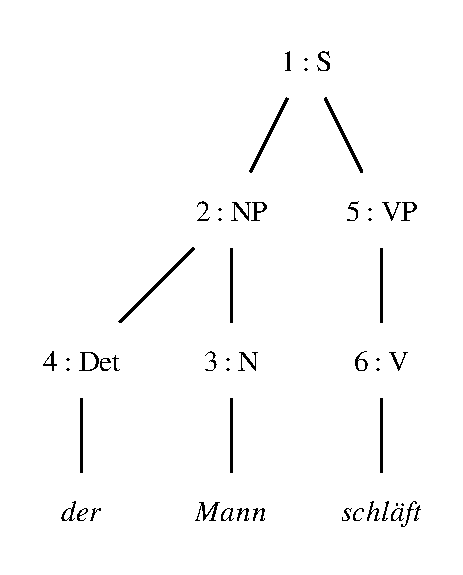
\includegraphics{minisatz/MiniSatzSyntax.eps}
\caption{Entsprechender Syntaxbaum}\label{CFG-Syntaxbaum}
\end{figure}
Im Formalismus des Grammatical Framework wird die oben gegebene Grammatik in die abstrakte und die konkrete Syntax zerlegt.
Dabei entspricht die abstrakte Syntax in etwa dem Syntaxbaum ohne die terminalen Blätter. Die abstrakte Syntax der kontextfreien Grammatik aus Beispiel \ref{CFG-Beispiel} ist in Listing \ref{GF-MiniSatzAbs} zu sehen. Zunächst gibt das Schlüsselwort \textbf{abstract} an, dass es sich um Datei mit einer abstrakten Syntaxbeschreibung handelt. Dieses Schlüsselwort wird vom Namen der Grammatik gefolgt. Anschließend folgt der Inhalt der Grammatik. \\
Zunächst werden mithilfe der \textbf{flags}-Direktive einige mögliche Einstellungen vorgenommen. In diesem sehr kurzen Beispiel wird nur die Startkategorie für das Parsing gesetzt, also die Wurzel aller Parsebäume. Andere mögliche Optionen sind z.B. die Einstellungen des Encodings und der Lexer, also das Programm, das die Eingabe in lexikalische Tokens zerlegt.\footnote{quelle} \\
Nach dem Schlüsselwort \textbf{cat} folgt eine Liste der nicht-lexikalischen Kategorien oder auch Nonterminal-Symbole. Sie entsprechen in etwa den Datentypen in (funktionalen) Programmiersprachen. \\
Hauptbestandteil der Grammatik sind offensichtlich die Syntaxregeln. Sie werden nach dem Schlüsselwort \textbf{fun} aufgelistet. Für denjenigen, der mit funktionaler Programmierung vertraut ist, kommt das Format der abstrakten Syntaxregeln möglicherweise bekannt vor, da es starke Ähnlichkeit zu Funktionensignaturen in Sprachen wie Standard ML oder Haskell hat. Dies ist allerdings kein Zufall, denn diese Regeln beschreiben lediglich die Bestandteile aus denen ein Ausdruck einer neuen Kategorie zusammengesetzt werden soll, ohne eine Aussage über das genaue Vorgehen zu treffen. Dies wird unabhänging voneinander in jeder konkreten Grammatik, die diese abstrakte Grammatik implementiert, beschrieben. So sagt die erste Regel mit dem Namen \texttt{mkNP} aus, dass ein Ausdruck der Kategorie \texttt{NP} aus einem Ausdruck der Kategorie \texttt{Det} und aus einem Ausdruck der Kategorie \texttt{N} zusammengesetzt werden kann. Die letzten drei Regeln führen lexikalische Einheiten mit einer entsprechenden Kategorie ein. \\
% Listing MiniSatzAbs
\lstinputlisting[float=ht,caption={Abstrakte Syntax},label={GF-MiniSatzAbs}]{minisatz/MiniSatzAbs.gf}
Diese abstrakte Grammatik kann nun konkret umgesetzt werden. Zwei konkrete Implementierungen, für Deutsch und Englisch, sind in Listing \ref{GF-MiniSatzGer} und \ref{GF-MiniSatzEng} zu finden. \\
% Listing MiniSatzGer
\lstinputlisting[float=ht,caption={Konkrete deutsche Syntax},label={GF-MiniSatzGer}]{minisatz/MiniSatzGer.gf}
% Listing MiniSatzEng
\lstinputlisting[float=ht,caption={Konkrete englische Syntax},label={GF-MiniSatzEng}]{minisatz/MiniSatzEng.gf}
Zunächst weist das Schlüsselwort \textbf{concrete} die Grammatik als eine konkrete Grammatik aus. Es folgt wie bei einer abstrakten Syntax der Name der Grammatik, diesmal wird jedoch darauf folgend angegeben welche abstrakte Grammatik die Grundlage bietet, hier unsere \texttt{MiniSatzAbs}-Grammatik. \\
Das in der deutschen, konkreten Grammatik verwendete Flag \texttt{coding} ermöglicht es, die Zeichenkodierung in den Zeichenketten festzulegen. In diesem Falle ist es für die deutschen Umlaute nötig das Encoding anzugeben.\footnote{quelle coding} Für andere Sprachen mit komplett vom lateinischen unterschiedlichen Schriftsystemen, gibt es auch die Möglichkeit statt der direkten Zeichenkodierung eine Transliteration zu verwenden.\footnote{quelle transliteration}\\
Das Schlüsselwort \textbf{lincat} ist die konkrete Entsprechung zum Schlüsselwort \textbf{cat} in der abstrakten Syntax. Hier müssen für jede in der abstrakten Syntax angegebene Kategorie ein konkreter Datentyp angegeben werden. In diesem Falle wurde für alle Kategorien der einfache Datentyp \texttt{Str}, also eine einfache Zeichenkette\footnote{Um genau zu sein, eine Liste von Tokens, die am Schluss mit Leerzeichen konkateniert werden}, gewählt. Das Grammatical Framework unterstützt auch verschiedene Arten komplexer Datentypen. \\
Auf den \texttt{lincat}-Block folgt, mit dem Schlüsselwort \texttt{lin} markiert, der Abschnitt, in dem die für jede abstrakte Syntaxregel beschrieben wird, wie diese in eine konkrete Zeichenkette zu übersetzen. Für die drei lexikalischen Regeln \texttt{Mann\_N}, \texttt{der\_Det} und \texttt{schlafen\_N} ist dies lediglich die entsprechende Zeichenkette z.B. für \texttt{Mann\_N} \textit{Mann} im Deutschen bzw. \textit{man} im Englischen. Die restlichen Syntaxregeln sind in diesem Beispiel nur geringfügig komplexer. Die Regel \texttt{mkVP} gibt lediglich den Parameter als Rückgabewert zurück, bildet also den gleichen String, der bereits als Parameter übergeben wurde. Und die beiden verbleibenden Regeln \texttt{mkNP} und \texttt{mkS} konkatenieren einfach die beiden als Parameter übergebenen Strings. \\
Man kann diese sehr kurzen konkreten Grammatiken zusammen mit der gemeinsamen Grammatik in das Grammatical Framework laden und in einer der beiden Sprachen den Satz \textit{der Mann schläft} bzw. \textit{the man sleeps} parsen und die abstrakte Representation \texttt{(mkS (mkNP der\_Det Mann\_N) (mkVP schlafen\_V))} in die andere Sprache linearisieren, also mit Hilfe der konkreten Syntaxregeln die entsprechende Zeichenkette in der Sprache generieren. \\
\begin{figure}
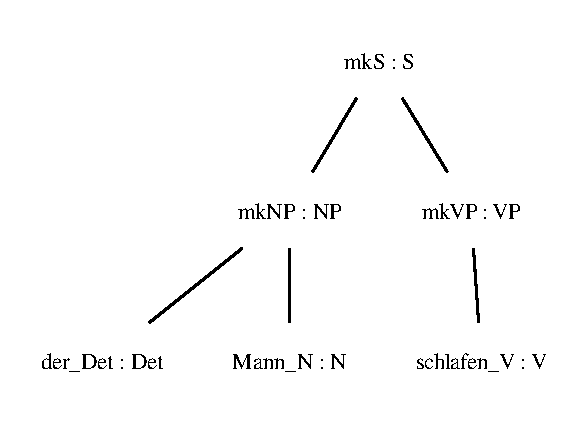
\includegraphics{minisatz/MiniSatzTree.eps}
\caption{Baum der abstrakten Syntax}\label{MiniSatz-AbsTree}
\end{figure}
\begin{figure}
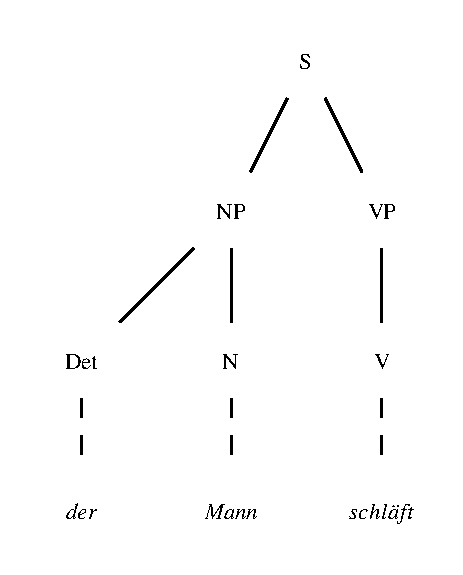
\includegraphics{minisatz/MiniSatzParseGer.eps}
\caption{Parsebaum der konkreten deutschen Syntax}\label{MiniSatz-ParseGer}
\end{figure}
Mit Hilfe des Grammatical Frameworks kann man auch verschiedene Bäume beim Parsen grafisch darstellen lassen. Zum einen den abstrakten Syntaxbaum und zum anderen den konkreten Parsebaum für eine der implementierten Sprachen. Diese Bäume für die MiniSatz-Grammatik sind in Abb. \ref{MiniSatz-AbsTree} und \ref{MiniSatz-Parse-Ger} zu sehen.
% Listing SatzAbs
\lstinputlisting[float=ht,caption={Erweiterte abstrakte Syntax},label={GF-SatzAbs}]{satz/SatzAbs.gf}
Nun kann man diese doch sehr minimalistische Grammatik etwas erweitern, so dass man auch die Sätze ``die Frauen schlafen'', ``der Mann sieht die Frau'' und ``der Mann liest das Buch''erkennen kann. Die fertigen Quelltextdateien sind in Listing \ref{GF-SatzAbs}, \ref{GF-SatzGer} und \ref{GF-SatzEng} zu finden. Die Veränderungen in der abstrakten Syntax (Listing \ref{GF-SatzAbs} sind nicht sehr umfangreich und betreffen hauptsächlich die Einführung von transitiven Verben mit der Kategorie \texttt{V2}. Mit der Funktion \texttt{mkVP2} wird aus einem transitiven Verb und einer Nominalphrase eine Verbalphrase mit Akkusativobjekt aufgebaut. Um auch Nominalphrasen im Plural zu ermöglichen, wird für den bestimmten Artikel eine Singular- und eine Pluralform benötigt. Sonst wird noch das ``Lexikon'' um die Wörter für Frau, Buch, sehen und lesen erweitert. \\
% Listing SatzGer
\lstinputlisting[float=ht,caption={Erweiterte konkrete deutsche Syntax},label={GF-SatzGer}]{satz/SatzGer.gf}
In der konkreten Umsetzung sind nun aber größere Unterschiede, sowohl zur ursprünglichen Grammatik, als auch zwischen den unterschiedlichen Sprachen zu finden. [fehlt: Beschreibung der konkreten Programme]
% Listing SatzEng
\lstinputlisting[float=ht,caption={Erweiterte konkrete englische Syntax},label={GF-SatzEng}]{satz/SatzEng.gf}
\FloatBarrier
\subsubsection{Die Ressource Grammar Library}
Was für allgemeine Programmiersprachen eine Standardbibliothek ist, ist im Grammatical Framework für die Multilingualität die Ressource Grammar Library. Sie ist definiert als gemeinsame abstrakte Syntax, die für verschiedenen Sprachen implementiert ist. Auf diese Möglichkeit ist eine grundlegende Übersetzung zwischen den unterstützten Sprachen direkt nach der Installation möglich. Meist muss jedoch mindestens das nötige Vokabular angegeben werden, da das Lexikon auf eine kleine Anzahl von Wörtern beschränkt ist, die benötigt wird um die grammatischen Konstrukte zu testen. \\
% Listing RglSatzAbs
\lstinputlisting[float=ht,caption={Abstrakte Syntax mit Hilfe der RGL},label={GF-RglSatzAbs}]{rglsatz/RglSatzAbs.gf}
% Listing RglSatzGer
\lstinputlisting[float=ht,caption={Konkrete deutsche Syntax mit Hilfe der RGL},label={GF-RglSatzGer}]{rglsatz/RglSatzGer.gf}
% Listing RglSatzEng
\lstinputlisting[float=ht,caption={Konkrete englische Syntax mit Hilfe der RGL},label={GF-RglSatzEng}]{rglsatz/RglSatzEng.gf}
\pagebreak
\FloatBarrier
\subsection{Die Lateinische Sprache}
\subsubsection{Sprachwissenschaftliche Einordnung}
Die lateinische Sprache, auch als oskisch-umbrische Sprache bezeichnet, gehört zur indogermanische Sprachfamilie und dort zur Unterfamilie der italischen Sprachen. Durch diese Verwandschaft kann man bei Wörtern und Wortformen oft Entsprechungen zwischen der lateinischen Sprache und verschiedensten anderen Sprachen Westeuropas bis hin zu Mittelasien finden (vgl. Tabelle \ref{Idg-Entsprechungen}.\footnote{vgl. BAYER-LINDAUER1994 S.1}
\begin{table}[h]
\begin{tabular}{|l|l|l|}
\hline
lateinisch & altgriechisch & deutsch \\
\hline
pater & \pi\alpha\tau\'{\eta}\rho\ (=patēr) & Vater \\
ager & \alpha\gamma\rho\'{o}\varsigma\ (=agr\'{o}s)& Acker \\
trēs & \tau\rho\varepsilon\~{\iota}\varsigma\ (=treĩs) & drei \\
decem & \delta\'{\varepsilon}\kappa\alpha\ (=d\'{e}ka) & zehn \\
\hline
\end{tabular}
\caption{Wortentsprechungen in verschiedenen indogermanischen Sprachen (vgl. BAYER-LINDAUER S.1)}
\label{Idg-Entsprechungen}
\end{table}
Entstanden ist es als ein in der Stadt Rom üblicher Dialekt parallel zu anderen ländlicheren Dialekten im Latium, im laufe der Zeit verdrängte es jedoch die weiteren italischen Sprachen im Zuge der Ausdehnung des römischen Reichs.\footnote{vgl. METZLER2004 S. 5359} Die Sprachgeschichte kann in mehrere Epochen unterteilt werden. Üblicherweise beginnt man diese Einordnung mit der Epoche des Altlateins, das von ca. 240 v. Chr bis 80 v. Chr angesiedelt wird. Es reicht von den frühesten nachgewiesenen lateinischen Sprachzeugnissen bis zum Beginn der Zeit des klassischen Lateins. Dessen Zeitaum wird von ca. 80 v. Chr. bis 117. n. Chr. gerechnet und beginnt in etwa mit den ersten öffentlichen Auftritten des M. Tullius Cicero. Die bekannten Gerichtsreden des berühmten römischen Anwalts und Schriftstellers von ca. 80 v. Chr sind noch größtenteils erhalten. Die nachklassische Phase kann wiederum in verschiedene Epochen unterteilt werden, in denen unter anderem die romanischen Volkssprachen entstanden sind, bis hin zum sogenannten Neulatein, das noch vom 15. Jahrhundert bis hin zum beginn des 20. Jahrhundert die Sprache der Wissenschaft darstellte und auch heute noch großen Einfluss auf Begriffe des Alltags ausübt.\footnote{MÜLLER-LANCE2006 S. 27ff.}  \\
Auch heute noch am bedeutendsten ist jedoch wohl das klassische Latein, das weiterhin in Schulen unterrichtet wird und sich vor allem mit seinem großen überlieferten Textkorpus hervorhebt. Da sich die meisten Lateingrammatiken auf diese Sprachepoche stützen, wird diese primär in dieser Arbeit betrachtet.\footnote{quelle}. \\
In der Sprachwissenschaft ist jedoch auch weiterhin umstritten, in welchem Verhältnis das klassische Latein zum sogenanten Vulgärlatein steht. Heutzutage geht man davon aus, dass das klasische Latein eine kaum wirklich gesprochene Sprache war und das Vulgärlatein nicht nur eine nachklassische Sprachvariante ist, sondern bereits parallel zum klasischen Schriftlatein als gesprochene Sprache verwendet wurde. Allerdings fand das klassische Latein noch bis in das 5. Jahrhundert n. Chr. Verwendung als eine Art Schreibnorm, während sich das Vulgärlatein langsam hin zu den romanischen Sprachen entwickelte.\footnote{vgl. METZLER2004 S. 5359 und S. 10719} \\
Formal gehört Latein den stark flektierenden Sprachen. Das heißt das in der lateinischen Sprache, wie für synthetische Sprachen üblich, syntaktische Klassen und Verhältnisse über Wortsuffixe ausgedrückt werden.\footnote{vgl. METZLER2004 S. 9690}. Allerdings drücken bei flektierenden Sprachen, im Gegensatz zu agglutinierenden Sprachen, die Affixe meist mehr als en grammatisches Merkmal aus.\footnote{vgl. METZLER2004 S. 3009} So ist bei der Verbform \textit{audio} das \textit{audi} der Verbstamm, um genau zu sein den Präsensstamm, des Verbs \textit{audire} und das Suffix \textit{-o} kodiert folgende Merkmale: 1. Person, Singular, Präsens, Indikativ, Aktiv.\footnote{vgl. BAYER-LINDAUER1994 S. 75} \\
Es gibt fünf zum Teil genusbasierte Flexionsklassen\footnote{Def. Flexionsklasse} für Nomen, sechs verschiedene Kasus (Nominativ, Genitiv, Dativ, Akkusativ, Ablativ und Vokativ), drei Genera (Maskulin, Feminin, Neutrum), ein voll flektierendes Pronomensystem und vier relativ stark synthetische Deklinationsklassen für Verben.\footnote{METZLER2004 S. 5359} Zu den Kasus sei anzumerken, dass der Ablativ im Lateinischen ein eigenständiger Kasus ist, jedoch der Vokativ oft mit dem Nominativ zusammenfällt.\footnote{vgl. BAYER-LINDAUER1994 S. 20f.} \\
Die Wortstellung des Lateinischen wird oft als sehr frei beschrieben, allerdings gibt es eine klare Präferenz der SOV-Wortstellung im Satz, also dass das Objekt des Satzes direkt auf das Subjekt folgt, und das Verb den Satz abschließt. Die Möglichkeiten zur Positionierung des Adjektivs im Bezug auf das Nomen sind allerdings durch nichts beschränkt.\footnote{METZLER2004 s. 5359}
\subsubsection{Bedeutung in der heutigen Zeit}
Man kann sich natürlich über die Notwendigkeit streiten, sich in der heutigen Zeit noch mit der lateinischen Sprache zu beschäftigen. Es gibt aber auch ziemlich gute Gründe dafür Latein nicht einfach nur als tote Sprache abzustempeln und nicht weiter zu betrachten. \\
Der am häufigsten, vor allem im Schulalter bei der Wahl einer zu lernenden Fremdsprache, vorgebrachte Grund ist, dass die lateinische Sprache als ``Mutter aller romanischen Sprachen'' später einen einfacheren Einstieg in das Erlernen z.B von Französisch oder Spanisch bietet. Auch gilt Latein galt seit Jahrhunderten, und gilt weiterhin, als produktive Quelle für Fachbegriffe aus Wissenschaft, Forschung und Technik. So haben viele moderne Begriffe wie Computer\footnote{von \textit{lat.} computere - berechnen} und Monitor\footnote{\textit{lat.} f. der Mahner, von \textit{lat.} monere - mahnen} lateinische Wurzeln. Auch im Universitätsalltat wird man oft mit lateinischen Lehnwörtern konfrontiert. Man trifft sich zum Essen in der Mensa\footnote{\textit{lat.} mensa - Tisch, Tafel} und studiert an Fakultäten\footnote{von \textit{lat.} facultas - Vermögen, Fähigkeit}. \\
Vor allem in der Sprachwissenschaft hat Latein eine besondere Bedeutung, da sie bei einem Vergleich verschiedener indogermanischer Sprachen als eine Art \textit{default}-Sprache angesehen werden kann, denn sie bietet fast alle nötigen grammatischen Kategorien, die gewöhnlich benötigt werden. So kann Latein als Vergleichsparameter (\textit{tertium comparationis}) verwendet werden. Diese Stellung der lateinischen Sprache spiegelt sich auch in der Fachterminologie moderner Schulgrammatiken wieder, die fast ausschließlich von lateinischen Fachausdrücken geprägt ist.\footnote{vgl. MÜLLER-LANCE2006 S. 10} \\
Als etwas skurile Verwendung einer Variation der lateinischen Sprache kann \textit{latino sine flexione} gelten. Diese von Giuseppe Peano anfang des 20. Jahrhunderts als Welthilfssprache entwickelte vereinfachte Form der lateinischen Sprache fand bis ca. 1950 in mehreren wissenschaftlichen Veröffentlichungen Verwendung. Sie basiert auf dem üblichen lateinischen Wortsschatz, der auch durch modernes romanisches Vokabular erweitert werden kann, und einer stark vereinfachten Morphologie.\footnote{vgl. METZLER2004 S. 5374}
\pagebreak
\section{Grammatikerstellung}
Nach der Einführung in die nötigen Grundlagen, um die Schritte zu verstehen, die nötig sind um im Grammatical Framework eine Grammatik zu entwickeln, folgt nun eine Schilderung der konkreten Schritte die nötig waren um eine Lateingrammatik im Grammatical Framework zu entwickeln. \\
Es sei noch anzumerken, dass es bereits früher Bestrebungen von Aarne Ranta gab, eine Lateingrammatik für die Ressource Grammar Library des Grammatical Frameworks zu entwickeln. Diese Arbeit baut auf diesen ersten Versuchen auf, kann aber insofern als selbständige und vollwertige Arbeit angsehen werden, da die bisherige implementierung sehr rudimentär war und seit ca. 2005 nicht mehr weiterentwickelt wurde. Im Anhang C ist der Quelltext meiner Arbeit als sogenanntes Diff\footnote{} zum Zustand vor Beginn der Arbeit zu finden. \\
Die Gliedering folgt dem gewählten Vorgehen bei der Implementierung. Die Begründung für die Reihenfolge der einzelnen Schritte wird jeweils zu Beginn der einzelnen Kapitel kurz dargelegt.
\subsection{Lexikon}
Den Beginn dieser Grammatikimplementierung bildete die Erstellung des minimal nötigen Lexikons. Durch die abstrakte Syntax der RGL\footnote{vgl. lib/src/abstract/Lexicon.gf und lib/src/abstract/Structural.gf} ist eine Liste von etwas über 450 englischen Bezeichnern für Worte vorgegeben, die in jeder Sprache umgesetzt werden sollten. \\
Für die Erstellung eines Lexikon, wie es in einer Grammatik verwendet werden kann, sind zwei Schritte nötig. Einerseits müssen für jeden vorgegebenen Bezeichner, in diesem Falle alle lexikalischen Funktionen aus dem abstrakten Lexikon die zugeordneten Zeichenketten zugeordnet werden. Und zum anderen muss das Lexikon auch all jene Informationen enthalten, die später zum bilden der Vollformen und zur Konstruktion grammatischer Einheiten nötig sind.
Der erste Schritt dabei begann damit, einfach das Lexikon einer anderen Sprache, in diesem Falle Englisch, zu kopieren. Normalerweise ist es vernünftiger, mit einer Sprache zu beginnen, die der zu implementierenden Sprache möglichst nahe steht.\footnote{RGL beginn}. Allerdings wurde diese Entscheidung vor Beginn meiner Arbeit getroffen, und ist insofern verständlich, da für die verwendeten Bezeichner in der Grammar Library bereits die englischen Begriffe zusammen mit einem Marker für die Wortart gewählt wurden. Anschließend wurden zunächst alle Zeichenketten durch mögliche lateinische Entsprechungen ersetzt. Um eine mögliche Übersetzung für die verschiedenen Lexikoneinträge zu finden, mussten verschiedene Vorgehensweisen angewandt werden. Hauptsächlich wurden, soweit möglich gedruckte Wörterbücher für die Übersetzung verwendet, gelegentlich waren aber auch Onlineresourcen unumgänglich. Des weiteren wird der Übersetzungsschritt von den englischen Bezeichnern zu den deutschen Entsprechungen, die für das weitere Vorgehen verwendet wurden, nicht genauer erläutert. Es sei nur so viel gesagt, dass die Bedeutung der meisten Begriffe ohne weitere Hilfsmittel ersichtlich war. Im Falle dessen, dass einmal Unklarheiten herrschten, wurde ein bekanntes Onlinewörterbuch\footnote{\url{http://dict.leo.org/}} verwendet.\\
\subsubsection{Wörterbücher}
Um eine passende lateinische Übersetzung für die Lexikoneinträge zu finden, wurde primär der deutsch-lateinische Teil eines handelsüblichen Schulwörterbuchs\footnote{Langenscheidt}, soweit ein entsprechender Eintrag im diesem Wörterbuch zu finden war. Allerdings gab es bereits an diesem Punkt diverse Herausforderungen. Denn eine Art von Wörtern, die allgemein zu Problemen bei der Übersetzung, und somit auch bei der Erstellung dieses Lexikons, führten, sind Wörter mit ambiger Bedeutung, wie das häufig als Beispiel angeführe Wort \textit{bank}, das in vielen Sprachen mehrere verschiedene Bedeutungen haben kann, z.B. im Deutschen als Sitzgelegenheit und als Geldinstitut oder im Englischen ebenfalls als Geldinstitut oder als Flussufer.\footnote{Quelle Ambig. Woerter} Für diesen und ähnliche Begriffe wurde willkürlich eine der plausiblen Bedeutungen gewählt, da keine Hinweise zur gewünschten Bedeutung in der Grammar Library gefunden werden konnte. Die Entscheidung eine einzige Bedeutung zu wählen, und nicht verschiedene Bedeutungen als Varianten des Wortes zu implementieren, wurde getroffen um die Anzahl der möglichen Übersetzungen möglichst gering zu halten. Für den Umgang mit ambigen Wörtern in einem Lexikon für das Grammatical Framework gibt es keine klaren Regeln, die angebrachteste Methode ist wohl, für jede Bedeutung einen eigenen Bezeichner zu wählen. So wäre z.B. \textit{bank1\_N} die Sitzgelegenheit und \textit{bank2\_N} das Geldinstitut.\\
Bei vielen, meist moderneren Begriffen, können jedoch nicht immer entsprechende Wörterbucheinträge gefunden werden. Zwar gibt es auch andere Wörterbücher, wie das Schulwörterbuch von PONS\footnote{PONS}, das einen umfangreicheren lateinisch-deutschen Teil enthält, und somit mehr moderne Begriffe abdeckt, allerdings gibt es auch dort Begriffe, für die auch hier kein Eintrag zu finden ist. Für diesen Fall müssen neben den bewährten gedruckten Wörterbüchern auch andere Quellen, vor allem Onlinequellen zu Rate gezogen werden.\\
\subsubsection{Onlinequellen}
Als Mögliche Lösung bietet sich die Nutzung von kollaborativen Internetquellen an. Eine der interessantes Quelle für moderne Begriffe aus dem Breich der Substantive ist wohl die lateinische Wikipedia\footnote{\url{http://la.wikipedia.org/wiki/Pagina\_prima}}. Obwohl Latein als tote Sprache gilt, existieren dort über 90000 lateinische Artikel\footnote{\url{http://la.wikipedia.org/wiki/Specialis:Census}; Stand: 30.7.2013}, die von einer recht Lebendigen Gemeinschaft gepflegt werden. Natürlich muss man immer bedenken, dass es keine Garantie für die Qualität von kollaborativen Onlinequellen gibt. Allerdings hat sich das Prinzip der Wikipedia ja auch in anderen Sprachen bewährt, wenn auch die Qualitätssicherung durch manuelle Korrekturen, und damit auch die Qualität der einzelnen Artikel, direkt von der größe der an dem Projekt arbeitenden Comunity zusammen. Neben der Wikipedia, die vom Konzept her eigentlich eine allgemeine Enzyklopädie ist, und nur im Nebeneffekt linguistische Resourcen zur verfügung stellt, gibt es noch weitere Internetquellen, die bei der Erstellung eines Lexikons helfen können. So gibt es das deutsche Lateinportal Auxilium-online.net\footnote{\url{http://www.auxilium-online.net/}}, das englischsprachige Wiktionary\footnote{\url{http://en.wiktionary.org/}} und die Lateinresourcen bei der Perseus Digital Libary\footnote{\url{http://www.perseus.tufts.edu/hopper/}}. \\
Das erstere bezeichnet sich selbst als das größte deutschsprachige Lateinportal im Internet und bietet ein kostenloses Onlinewörterbuch, sowohl in der Richtung Lateinisch-Deutsch als auch umgekehrt, das von registrierten Benutzern erweitert und korrigiert werden kann. Allerdings liegt bei diesem Wörterbuch der Schwerpunkt auch eher auf dem klassischen Vokabular. \\
Das englischsprachige Wiktionary hilft zwar nicht direkt bei der Suche nach einer direkten Übersetzung aus einer anderen Sprachee, es bietet aber für ein umfangreiches Vokabular sowohl eine morphologische Analyse für viele Wortformen als auch detailierte Informationen über Verwendung und Formenbildung für lateinische Vokabeln. \\
Die Perseus Digital Library, und vor allem die darin enthaltenen Wörterbücher fallen eher in die Kategorie klassischer, gedruckter Wörterbücher, was primär daher rührt, dass diese Wörterbücher Digitalisate seit Jahrzehnten bewährter Wörtrebücher sind.\footnote{\textit{A Latin Dictionary. Founded on Andrews' edition of Freund's Latin dictionary. revised, enlarged, and in great part rewritten by. Charlton T. Lewis, Ph.D. and. Charles Short, LL.D. Oxford. Clarendon Press. 1879.} (\persalatin) und \textit{Lewis, Charlton, T. An Elementary Latin Dictionary. New York, Cincinnati, and Chicago. American Book Company. 1890.} (\perselemlat)} Jedoch bietet Perseus die Möglichkeit einer erweiterten Suchfunktion so wie einer Angabe zur Wortfrequenz im verfügbaren Korpus. \\
Eine der Onlinequellen für moderne lateinische Begriffe wurde nicht verwendet, da sie nur zwischen Latein und Italienisch übersetzt. Dies würde aus verschiedenen Gründen zu Problemen führen. Diese Quelle soll allerdings trotzdem kurz erwähnt werden, denn sie ist die offizielle Liste des Vatikans zur Übersetzung moderner Alltagsbegrifft\footnote{\vatlatinitas}.
\subsubsection{Geschlossene Kategorien}
Das Lexikon einer Ressource Grammar ist unterteilt in zwei Dateien. Die erste Datei, StructuralLat.gf, enthält die Einträge für die sogenannten geschlossenen Kategorien, so wie einige weiter Einträge die eher eine strukturelle als eine lexikalische Bedeutung haben. Die meisten Wortarten in diesem Teil des Lexikons gehören zu den sogenannten Partikeln, die nicht flektiert werden. Dazu gehören vor allem Adverbien, Präpositionen und Konjunktionen.\footnote{BAYER-LINDAUER1994 S.12} \\
Adverbien gehören eigentlich nicht wirklich zu den geschlossenen Kategorien, jedoch gibt es eine gewisse Anzahl von Adverbien und adverbial benutzten Wörtern, die den meisten Sprachen gemein sind, weswegen sie als strukturale Bestandteile aufgefasst werden können. Meist werden Adverbien aus Adjecktiven gebildet, weswegen man sie zu den offenen Kategorien rechnen sollte. Jedoch ist dies nur eine von verschiedenen Möglichkeiten zur Verwendung von Adverbien. Vor allem im  Bereich der lokalen Adverbien (auf die Fragen wo?, wohin?, woher?) gibt es nur ein eingeschränktes Vokabular, das zu Recht zu den geschlossenen Kategorien gerechnet werden kann.\footnote{BAYER-LINDAUER1994 S.44} 
Konkret als \texttt{Adv}\footnote{verb-phrase-modifying adverb \url{http://www.grammaticalframework.org/lib/doc/synopsis.html#Adv}} gekennzeichnet, sind im Falle der Ressource Grammar Library die Bezeichner \texttt{everywhere\_N},\texttt{here\_Adv},\texttt{here7to\_Adv}, \texttt{here7from\_Adv}, \texttt{somewhere\_Adv}, \texttt{there\_Adv}, \texttt{there7to\_Adv} und \texttt{there7from\_Adv}. Betrachtet man die Übersetzung dieser Bezeichner, so stellt sich heraus, dass die lateinischen Wörter \textit{ubique}, \textit{hic}, \textit{huc}, \textit{hinc}, \textit{usquam}, \textit{ibi}, \textit{eo} und \textit{inde} in der Lateingrammatik nicht als Adverbien, sondern als Pronominaladverbien, aufgeführt werden, also eher zur geschlossenen Kategorie der Pronomen, allerdings mit adverbialer Verwendung gehören. \\
Zur selben grammatischen Kategorie gehören die meisten der im Grammatical Framework als \texttt{IAdv}\footnote{interrogative adverb \url{http://www.grammaticalframework.org/lib/doc/synopsis.html#IAdv}} bezeichneten Vokabeln \texttt{how\_IAdv} (lat. \textit{qui}), \texttt{when\_IAdv} (lat. \textit{quando}) und \texttt{where\_IAdv} (lat. \textit{ubi}). Das Wort \texttt{how8much\_IAdv} (lat. \textit{quantum}) wird als korrellatives Pronomen bezeichnet, lediglich das Fragewort \texttt{why\_IAdv} (lat. \textit{cur}) ist in der gegebenen Grammatik nicht explizit eingeordnet, hat aber offensichtlich eine verwandtschaftliche Beziehung zu (Interrogativ-)Pronomen\footnote {vgl. wer? -  lat. \textit{quis}, Dat. \textit{cur}}.
%less_CAdv = mkCAdv "minus" "quam"
%more_CAdv = mkCAdv "magis" "quam"
%as_CAdv = mkCAdv "ita" "ut"
%???
%quite_Adv = ss "admodum"

Prepositions


\FloatBarrier
\subsubsection{Offene Kategorien}
Das Lexikon der offenen Kategorien LexiconLat.gf ethält eine kleine Anzahl aus Wörtern aus den sogenannten offenen Kategorien, vornehmlich Nomen, Verben und Adjektive. 
Die Einträge haben unterschiedliche Umfang. Dies ist zum einen abhängig von der Menge an Informationen, die nötig ist um das gesamte Paradigma des generieren. Wovon dies abhängig ist wird im Kapitel über die Morphologie genau beschrieben. Im allgemeinen reicht, bei regelmäßiger Deklination\footnote{Nomenflektion} und Konjugation\footnote{Verbflexion}, eine einzelne Zeichenkette aus. \\
Die meisten Zeichenketten konnten, wie bereits erläutert wurde
\subsubsection{Ausnahmen} 
\pagebreak
\subsection{Morphologie}
Eine der großen Herausforderung bei der Implementierung einer Lateingrammtik, ist die Morphologie. Dies bedingt daraus, dass Latein eine flektierende Sprache ist, und deshalb viele grammatische Merkmale in der Wortform kodiert. Dadurch beding ist eine große Menge an Wortformen für jeden Lexikoneintrag. Um so wichtiger ist es, möglichst viele dieser Formen mit möglichst wenig Informationen zu generieren. Deshalb ist es ratsam, das Konzept der sogenannten Smart Paradigms zu implementieren. Dabei wird versucht Mit Hilfe von Stringanalysen möglichst viele Informationen zur Wortbildung zu extrahieren. Im Falle der lateinischen Sprache werden dabei Wortsuffixe zu Rate gezogen.
\subsubsection{Nomenflektion}
In der lateinischen Sprache gibt es fünf deklinationsklassen für Nomen. Sie werden entweder durchnummeriert oder aber durch ihren Kennlaut bestimmt. Demnach unterscheidet man die erste bis fünfte Deklination bzw. die ā-, ǒ-, ǐ-, ǔ- und ē-Deklination. Den zur Identifikation kann man den Kennlaut am leichtesten nach Abtrennung der Endung \textit{-um} im Genitiv Plural erkennen. \footnote{BAYER-LINDAUER1994 S. 21}\\
Allerdings kann man meist die Deklinationsklasse auch an der Endung der Nominativ Singular Form erkennen. So haben z.B alle Nomen der ā-Deklination den Ausgang \textit{-ǎ} und Genus Femininum. Es gibt keine wirklich relevanten Ausnahmen, so können lediglich Flußnamen und männliche Personennamen männliches Geschlecht haben. Deshalb ist es bei fast allen Nomen dieser Deklinationsklasse nicht nötig mehr als die Nominativ Singular Form anzugeben. \\
Bei der zweiten Deklinationsklasse gibt es eine größere Anzahl möglicher Wortausgänge, nämlich \textit{-us}, \textit{-um} und \textit{-er} bzw. \textit{-ir}. Grundätzlich sind Nomen mit dem Ausgang \textit{-um} Neutra, Nomen mit den Endungen \textit{-us} und \textit{-r} Maskulina. \\
Die dritte oder auch ǐ-Deklination wird auch als Mischdeklination bezeichnet, da sie in zwei Unterklassen unterteilt werden kann, in Nomen mit konsonantischem oder vokalischem, also auf \textit{-ǐ} auslautendem Stamm. Auf Grund dessen gehört die dritte Deklination zu den schwerer zu handhabenden Flexionsklassen. In Folge dessen reicht auch nicht eine einzige Wortform für die Generierung des Paradigmas aus. [todo: blablabla] \\
Die vierte Deklinationsklasse hingegen ist wieder unkomplizierter. Sie hat im Nominativ Singular die Endungen \textit{-ū} oder \textit{-us} und die Nomen sind, wenn sie auf \textit{-us} enden, maskulin und, wenn sie auf \textit{-ū} enden, Neutra. Da die Nominativ Singular Form bei den Nomen auf \textit{-us} nicht von Nomen der zweiten Deklination mit der gleichen Endung zu unterscheiden sind, kann das Smart Paradigm für nur eine Wortform nur bei den Nomen auf \textit{-ū} angewadt werden, da die Endung \textit{-us} schon die zweite Deklination identifiziert. In diesem Falle wird ebenfalls das Paradigma mit Hilfe den drei Parameter Nominativ Singular, Genitiv Singular und Geschlecht bestimmt. \\
Bei der fünften Deklination ist die Nominativ Singular-Endung an sich wieder eindeutig, sie enden alle auf \textit{-es}. Jedoch können, wie oben bereits beschrieben, auch Nomen der dritten Deklination im Nominativ Singular auf \textit{-es} enden. Man kann die unterschiedlichen Deklinationen aber klar an der Genitiv Singular-Form unterscheiden. Deshalb ist die sicherste Möglichkeit Fehler zu vermeiden, auch diese Genitivform im Lexikon anzugeben. Dies ist jedoch nicht nötig, da wenn nur die Nominativform angegeben ist und diese auf \textit{-es} endet, das Smart Paradigm so definiert ist, dass ein Paradigma der fünften Deklination generiert wird. \\
Die Bildung der Wortformen für Nomen ist fast schon trivial. Der Wortstamm wird meist dadurch gefunden, dass man, wenn nötig, die Endung abtrennt. Anschließend werden alle zwölf Wortformen, für die zwei Numeri und die sechs Kasus, durch anfügen der passenden Endung gebildet. \\
Bei der ersten Deklination ist der Wortstamm angenehmerweise gleich der Nominativ Singular-Form. Ebenfalls identisch zum Wortstamm sind die Ablativ und Vokativ Singular-Formen. Die Endungen für die restlichen Kasus sind \textit{-m} für den Akkusativ Singular, \textit{-e} für den Genitiv und Dativ Singular so wie Nominativ und Vokativ Plural, \textit{-rum} für den Genitiv Plural, und \textit{-s} für Akkusativ Plural. Etwas anders verhält es sich bei Dativ und Ablativ Plural. Bei diesen zwei Fällen wird die Endung \textit{-is} nicht an den Wortstamm, sondern an den Wortstock, also den Wortstamm, ohne den Kennvokal, angefügt.\footnote{BAYER-LINDAUER1994 S.21f.} \\
\begin{table}[h]
\begin{tabular}{|r:c:l|}
\hline
\multicolumn{2}{|l:}{Wortstamm} & Endung \\
\hline
terr & a & e \\
\hline
Wortstock & \multicolumn{2}{:l|}{Wortausgang} \\
\hline
\end{tabular}
\caption{Bestandteile eines lateinischen Nomens im Genitiv Singular (Vgl. BAYER-LINDAUER S. 21)}
\end{table}
Bei der zweiten Nomendeklination ist das Vorgehen ganz ähnlich zur ersten Deklination, zumindest bei den Nomen auf \textit{-us} und \textit{-um}. Diesmal muss von der Nominativ Singular-Form die Endung abgespalten werden um, diesmal den Wortstock, zu erhalten. An diesen werden nun die kasusabhängigen Ausgänge angehängt. Diese sind in den meisten Fällen für alle Nomen dieser Deklinationsklasse gleich, in manchen Kasus unterscheiden sie sich aber je nach Nominativ Singular-Endung. Somit ist logischerweise der Nominativ Singular nicht einheitlich sondern hat die Endungen \textit{-us}, \textit{-um} oder \textit{-r}. Die gleichen Endungen haben all diese Nomen im Genitiv, Dativ, Akkusativ und Ablativ Singular (\textit{-i}, \textit{-o}, \textit{-um}, \textit{-o}) sowie im Genitiv, Dativ und Ablativ Plural (\textit{-orum}, \textit{-is} und \textit{is}). 
\subsubsection{Verbdeklination}
\subsubsection{Pronomen}
\subsubsection{Ausnahmen}
\pagebreak
\subsection{Syntax}
\subsubsection{Nominalphrasen}
\subsubsection{Verbalphrasen}
\subsubsection{Einfache Sätze}
\pagebreak
\section{Ausblick}
\pagebreak
\section*{Bibliographie}
\pagebreak
\section*{Anhang}
\subsection*{Quelltext}
%\lstinputlisting[float=ht,caption={Konkrete englische Syntax mit Hilfe der RGL},label={GF-RglSatzEng}]{complete.diff}
\end{document}
